\chapter{Motion Law}%
\label{chap:motion_law}

	The path found with the algorithms described in
	Chapter~\ref{chap:path_processing} can be considered as a continuous smooth
	mapping that adheres to:

	\begin{equation}
		\pathsym : \timenorm \in [0, 1] \mapsto \specialEuclideanGroup{3}
			\quad
			\suchthat
			\quad
			\pathsym(0) = \pose_{\initial}, \pathsym(1) = \pose_{\goal},
			\forall\obstacle\forall(\pose\in\pathsym)
				\robot(\pose) \cap \obstacle = \emptyset
	\end{equation}

	If $\timenorm$ is interpreted as time, then it would imply that the robot is
	in its initial pose at $\timesym = 0\si{\second}$ and reaches its goal pose
	at $\timesym = 1\si{\second}$. While $\pathsym$ is guaranteed to be free of
	collisions, this interpretation makes no guarantee that the actuators can
	move the end-effector this fast. For this reason, a motion law,
	$\motionlaw$, must be found that performs the following mapping:

	\begin{equation}
		\motionlaw: \timesym\in\Re \mapsto \timenorm\in[0, 1]
	\end{equation}

	The trajectory, $\traj:\timesym \mapsto \specialEuclideanGroup{3}$, can then
	be defined simply as:

	\begin{equation}
		\traj = \pathsym(\motionlaw(\timesym))
	\end{equation}

	In addition to the no-collision guarantees of $\pathsym$, $\traj$ also
	guarantees that the actuators stay within their saturation ranges. The
	present chapter describes the approach followed to find a suitable
	$\motionlaw$. Sections~\ref{sec:motion_law_generation_algorithm}
	and~\ref{sec:ensuring_a_smooth_start} describe the procedure developed with
	schematic illustrations.
	Section~\ref{sec:sample_motion_law_processing_output} confirms the
	algorithms with numerically generated graphs.

	\section{Motion Law Generation Algorithm}%
\label{sec:motion_law_generation_algorithm}

	Since the actuators work directly on the length of the cables, the
	search for a suitable motion law $\motionlaw$ is performed in cable
	space and not in pose space. As a first step, $\timenorm$ is considered
	to be linked directly to time, $\timesym \defeq \timenorm$, and the
	cable velocities along the resulting trajectory is then found as:

	\begin{equation}
		\dot{\cablevec}(\timenorm) =
			\invgeometricmodel
			\left(
				\frac
				{%
					\der\pathsym
				}
				{%
					\der\timesym
				}
			\right)
	\end{equation}

	Each cable in $\cablevec$ is subjected to kinematic constraints on its
	velocity, $\dot\cablelength_{\max}$.  That is, each cable has a maximum
	velocity which it may not exceed. As such, the next step in the algorithm is
	finding the ranges that exceed this maximum velocity. In other words, find
	the set of time instants $\timenorm$ where:

	\begin{equation}
		\abs{\dot{\cablevec}(\timenorm)} \geq \dot{\cablevec}_{\max}
		\label{eq:excessive_cable_velocity}
	\end{equation}

	In general, there may be multiple ranges along the trajectory where the
	maximum velocity in Equation~\ref{eq:excessive_cable_velocity} is
	exceeded. A range in $\timenorm$, $\rangetimenorm$, is encapsulated as
	the ordered tuple:

	%\begin{equation}
	%	\rangetimenorm =
	%		\left(
	%			\timenorm_{\min},
	%			\timenorm_{\max}
	%		\right)
	%	%
	%\end{equation}

	%such that

	%\begin{equation}
	%	\abs
	%	{%
	%		\dot{\cablevec}
	%			(
	%				\timenorm
	%			)
	%	}
	%	%
	%	\geq \dot{\cablevec}_{\max}
	%	\quad
	%	\forall\timenorm\in[\timenorm_{\min}, \timenorm_{\max}]
	%\end{equation}

	%and

	%\begin{align}
	%	\begin{split}
	%		\dot{\cablevec}(\timenorm_{\min}^-) &< \dot{\cablevec}_{\max} \\
	%		\dot{\cablevec}(\timenorm_{\min}^+) &> \dot{\cablevec}_{\max} \\
	%		\dot{\cablevec}(\timenorm_{\max}^-) &> \dot{\cablevec}_{\max} \\
	%		\dot{\cablevec}(\timenorm_{\max}^+) &< \dot{\cablevec}_{\max} \\
	%	\end{split}
	%\end{align}

	\begin{equation}
		\rangetimenorm =
			\left(
				\timenorm_{\min},
				\timenorm_{\max}
			\right)
		%
		\quad
		\suchthat
		\quad
		%
		\begin{cases}
			\abs
			{%
				\dot{\cablevec}
					(
						\timenorm
					)
			}
			\geq \dot{\cablevec}_{\max}
			\forall\timenorm\in[\timenorm_{\min}, \timenorm_{\max}]\\
			%
			\dot{\cablevec}(\timenorm_{\min}^-) < \dot{\cablevec}_{\max} \\
			\dot{\cablevec}(\timenorm_{\min}^+) > \dot{\cablevec}_{\max} \\
			\dot{\cablevec}(\timenorm_{\max}^-) > \dot{\cablevec}_{\max} \\
			\dot{\cablevec}(\timenorm_{\max}^+) < \dot{\cablevec}_{\max} \\
		\end{cases}
	\end{equation}

	Note that the following notation is used to test whether a value is in a
	range:

	\begin{equation}
		\timenorm \in \rangetimenorm =
			\begin{cases}
				\true, \quad \timenorm \in [\timenorm_{\min},
				\timenorm_{\max}] \\
				\false, \quad\text{otherwise}
			\end{cases}
	\end{equation}

	All such ranges are put into an ordered set of ranges,
	$\setofrangestimenorm$, such that:

	\begin{equation}
		{\rangetimenorm}_{\indexi} \prec
		{\rangetimenorm}_{\indexj} \iff
		{\rangetimenorm}_{\indexi}\code{.}{\timenorm_{\max}} <
		{\rangetimenorm}_{\indexj}\code{.}{\timenorm_{\min}}
	\end{equation}

	$\setofrangestimenorm$ is then used as an input to the algorithms that
	generate $\motionlaw$.

	The idea behind the algorithm is now to simply scale the time in such a
	way that:

	\begin{equation}
		\frac
		{%
			\der\timesym
		}
		{%
			\der\timenorm
		}
		=
		\begin{cases}
			1, \quad \timenorm \notin \setofrangestimenorm \\
			\gain_{\indexi}, \quad \timenorm \in {\rangetimenorm}_{\indexi}
		\end{cases}
		\forall{\rangetimenorm}_{\indexi}\in\setofrangestimenorm
	\end{equation}

	Where $\gain_{\indexi}$ is chosen such that, for the currently active
	${\rangetimenorm}_{\indexi}$:

	\begin{equation}
		\abs
		{%
			\dot{\cablevec}(\timenorm)
		}
		\leq \dot{\cablevec}_{\max}
		\quad\forall{\timenorm}\in{\rangetimenorm}_{\indexi}
	\end{equation}

	A graphical intuition of the algorithm is given in
	Figure~\ref{fig:motion_law_graphical_intuition}. The top graph shows the
	velocity profile of a single cable for a given path
	$\pathsym(\timenorm)$. It also highlights the set $\setofrangestimenorm$
	that exceed the maximum velocities. The middle graph shows schematically
	how the motion law $\motionlaw:\timesym \mapsto \timenorm$ is
	generated. Finally, the bottom graph shows the effect of applying
	$\motionlaw$ to $\pathsym$ to obtain a trajectory $\traj(\timesym)$
	which no longer exceeds maximum velocities.

	\begin{figure}[hb]
		\centering
		\def\svgheight{8cm}
		\import{res/img/}{motion_law_intuition.pdf_tex}
		\caption{Motion Law Construction}%
		\label{fig:motion_law_graphical_intuition}
	\end{figure}

	The motion law shown in Figure~\ref{fig:motion_law_graphical_intuition} will
	guarantee that the velocity constraints of the actuators are respected.
	However, the corners in this graph correspond to sudden changes in the rate
	at which $\pathsym$ is followed and can lead to excessive accelerations in
	the cables. For this reason, instead of using the motion law as it is
	presented in Figure~\ref{fig:motion_law_graphical_intuition}, the corners
	are used as control points of the form $\mlcontrolpoint = \left(\timesym,
	\timenorm\right)$. The set of these points is denoted $\mlcontrolpointset$.
	These control points can then be interpolated using a B-spline of sufficient
	degree. A B-spline of degree two can guarantee continuous accelerations.
	Higher-degree B-splines guarantee continuity in higher time derivatives of
	$\traj$. A graphical representation of a B-spline motion law is shown in
	Figure~\ref{fig:motion_law_spline}.

	\begin{figure}[hb]
		\centering
		\def\svgwidth{\textwidth}
		\import{res/img/}{motion_law_spline.pdf_tex}
		\caption{Motion Law B-Spline Interpolation}%
		\label{fig:motion_law_spline}
	\end{figure}

	When interpolating the motion law with a B-spline, certain segments of the
	motion law may have a steeper slope than the corresponding segments of the
	linear interpolation of the control points. A steeper slope means in the
	motion law corresponds to faster progression along the trajectory and
	therefore higher cable velocities than those provided by the base linear
	interpolation.  Figure~\ref{fig:augmented_motion_law_control_points}
	highlights the areas of the motion law of Figure~\ref{fig:motion_law_spline}
	that have a higher slope. These areas correspond to regions where the output
	velocities may violate the constraints. To combat this, the control points
	may be augmented in a manner similar to
	Algorithm~\ref{alg:set_of_poses_augmentation}. The output of this is
	illustrated schematically on the right hand side of
	Figure~\ref{fig:augmented_motion_law_control_points}. The effect of such a
	procedure is to follow the base motion law as closely as possible, but then
	connect the sharp corners with smooth bends.

	\begin{figure}[hb]
		\centering
		\def\svgwidth{\textwidth}
		\import{res/img/}{motion_law_spline_problem.pdf_tex}
		\caption{Augmented Motion Law Control Points}%
		\label{fig:augmented_motion_law_control_points}
	\end{figure}

	There is one issue with using a B-spline in this context, however. Each
	control point for the spline is a coordinate in
	\(
		\left(
			\timesym, \timenorm
		\right)
	\)-space. The B-spline $B$ is a mapping of some variable $x$:

	\begin{equation}
		B: x \in [0, 1] \mapsto \left(\timesym, \timenorm\right)
	\end{equation}

	However, for use with a motion law, an explicit formula of the form

	\begin{equation}
		\timenorm = \timenorm(\timesym)
		\label{eq:direct_relation_motion_law_spline}
	\end{equation}

	is required. To obtain this explicit form, three options are available:

	\begin{enumerate}

		\item

			Rewrite Equation~\ref{eq:b_spline_recursion} in a non-implicit form.
			\label{option:rewrite_non_implicit}

		\item

			Solve for
			\(
				x = \function(\timesym)
			\)
			using numerical techniques such as Newton's method or Regula
			Falsi. Then obtain
			\(
				\timenorm = g(x) = g(\function(\timesym))
			\)
			from there.
			\label{option:solve_numerically}

		\item

			Build a lookup table and smoothly interpolate.
			\label{option:lookup_table}

	\end{enumerate}

	It would clearly be ideal to have a direct relation as in
	Equation~\ref{eq:direct_relation_motion_law_spline}. However,
	Option~\ref{option:rewrite_non_implicit} requires expensive computations and
	difficult to implement algorithms.

	Option~\ref{option:solve_numerically} would require that an implicit
	equation be solved each time the motion law is evaluated. This is not ideal
	when the trajectory is used for robot control.

	For these reasons, this thesis makes uses of the lookup table approach in
	Option~\ref{option:lookup_table}. This is achieved by creating an ordered
	set of pairs

	\begin{equation}
		\set{T} =
		\left\{
			(\timesym_0, \timenorm_0),
			\ldots,
			(\timesym_n, \timenorm_n)
		\right\}
	\end{equation}

	upon creation of the motion law. This is done by defining a discrete set
	$\set{X}$ that spans the domain $x$ of $B$ with
	linearly spaced intervals. $\set{T}$ is then found simply by the relation
	\(
		\set{T} = B(\set{X})
	\).

	The motion law is then approximated by:

	\begin{equation}
		\motionlaw(\timesym) \approx
			\timenorm_{\indexi} +
				\frac
				{%
					\timesym - \timesym_{\indexi}
				}
				{%
					\timesym_{\indexi + 1} - \timesym_{\indexi}
				}
				\left(
					\timenorm_{\indexi + 1} - \timenorm_{\indexi}
				\right)
	\end{equation}

	Where

	\begin{equation}
		\timesym \in [\timesym_{\indexi}, \timesym_{\indexi + 1}]
	\end{equation}

	Using a lookup table did not lead to any noticeable impacts on the
	speed of execution, even when a large number of samples was taken to build
	a high-resolution lookup table. This justifies using the simplification of
	Option~\ref{option:lookup_table} instead of the exactness of
	Option~\ref{option:rewrite_non_implicit}.


	\section{Ensuring a Smooth Start}%
\label{sec:ensuring_a_smooth_start}

	Consider again Figure~\ref{fig:augmented_motion_law_control_points}. The
	algorithm as presented in Section~\ref{sec:motion_law_generation_algorithm}
	will have a tendency to produce infinite accelerations at $\timesym = 0$.
	This is due to the fact that the slope of the B-spline-interpolated motion
	law at $\timesym = 0$ is non-zero and thus represents a loss of
	differentiability analogous to the loss of differentiability in the
	piecewise linear motion law illustrated in the left half of
	Figure~\ref{fig:motion_law_spline}.

	To combat this effect, an acceleration phase may be introduced into the
	motion law. The goal of this phase is to prepend a section that smoothly
	interpolates from zero slope to the initial slope of the original motion
	law. This is done by choosing some acceleration period $\Delta\timesym$ and
	changing the control points according to:

	\begin{equation}
		\timesym_{\indexi} \gets \timesym_{\indexi} + \Delta\timesym
			\quad\forall\timesym_{\indexi} \in \mlcontrolpointset \setminus \timesym_0
	\end{equation}

	This can be seen as shifting all but the first control point further into
	time. Now, a new control point $\mlcontrolpoint'$ must be created subject
	to:

	\begin{align}
		\begin{split}
			\mlcontrolpoint'.\timesym &\in (0, \Delta\timesym)\\
			\mlcontrolpoint'.\timenorm &\in (0, \mlcontrolpoint_1.\timenorm)
		\end{split}
	\end{align}

	$\mlcontrolpoint'$ is then inserted into $\mlcontrolpointset$ between
	$\mlcontrolpoint_0 $ and $\mlcontrolpoint_1$. To ensure that the slope
	during the acceleration phase of the motion law contains a near-horizontal
	section of sufficient length, the following values are used in this thesis:

	\begin{align}
		\begin{split}
			\mlcontrolpoint'.\timesym &= 0.9\Delta\timesym\\
			\mlcontrolpoint'.\timenorm &= 0.1\mlcontrolpoint_1.\timenorm
		\end{split}
	\end{align}

	The effect of applying this procedure is shown schematically in
	Figure~\ref{fig:smooth_start_motion_law_construction}. Although this figure
	intends to give only a graphical intuition, it is drawn using B-spline
	curves. As can be seen in the figure, this procedure effectively shifts the
	entire motion law in time and slowly accelerates the motion law from zero
	slope to its initial slope.

	\begin{figure}[hbt!]
		\centering
		\def\svgwidth{\textwidth}
		\import{res/img/}{acceleration_phase.pdf_tex}
		\caption{Smooth Start Motion Law Construction}%
		\label{fig:smooth_start_motion_law_construction}
	\end{figure}

	\todo{Next section needs to be updated with figures generated using the
	approach of this section}

	\section{Sample Motion Law Processing Output}%
\label{sec:sample_motion_law_processing_output}

	The current section shows and discusses sample output of the algorithm
	described in Section~\ref{sec:motion_law_generation_algorithm}. The current
	discussion relates to the planning problem and trajectory of
	Figure~\ref{fig:motion_law_sample_problem}.

	\begin{figure}[hb]
		\begin{minipage}{0.5\textwidth}
			\centering
			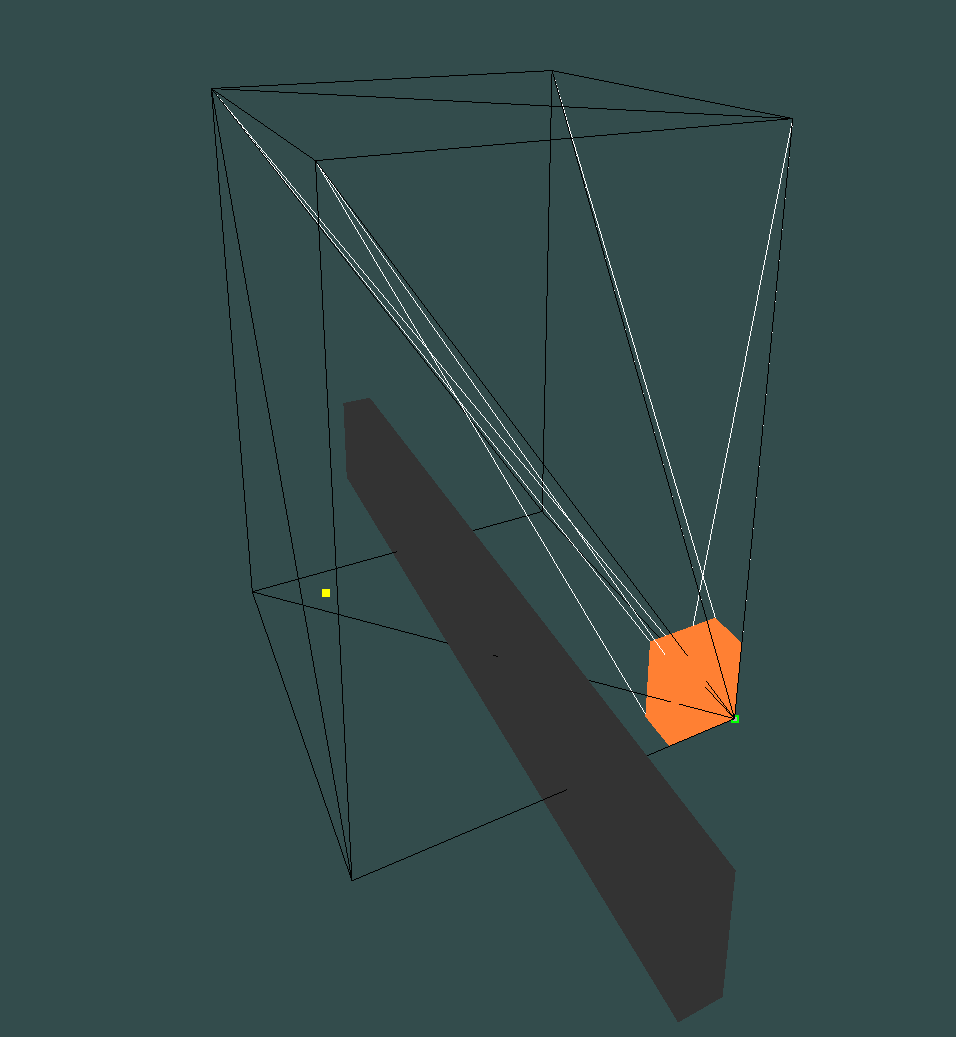
\includegraphics[height=0.6\textwidth]{kinematic_scaling_base_problem}
		\end{minipage}
		\begin{minipage}{0.5\textwidth}
			\centering
			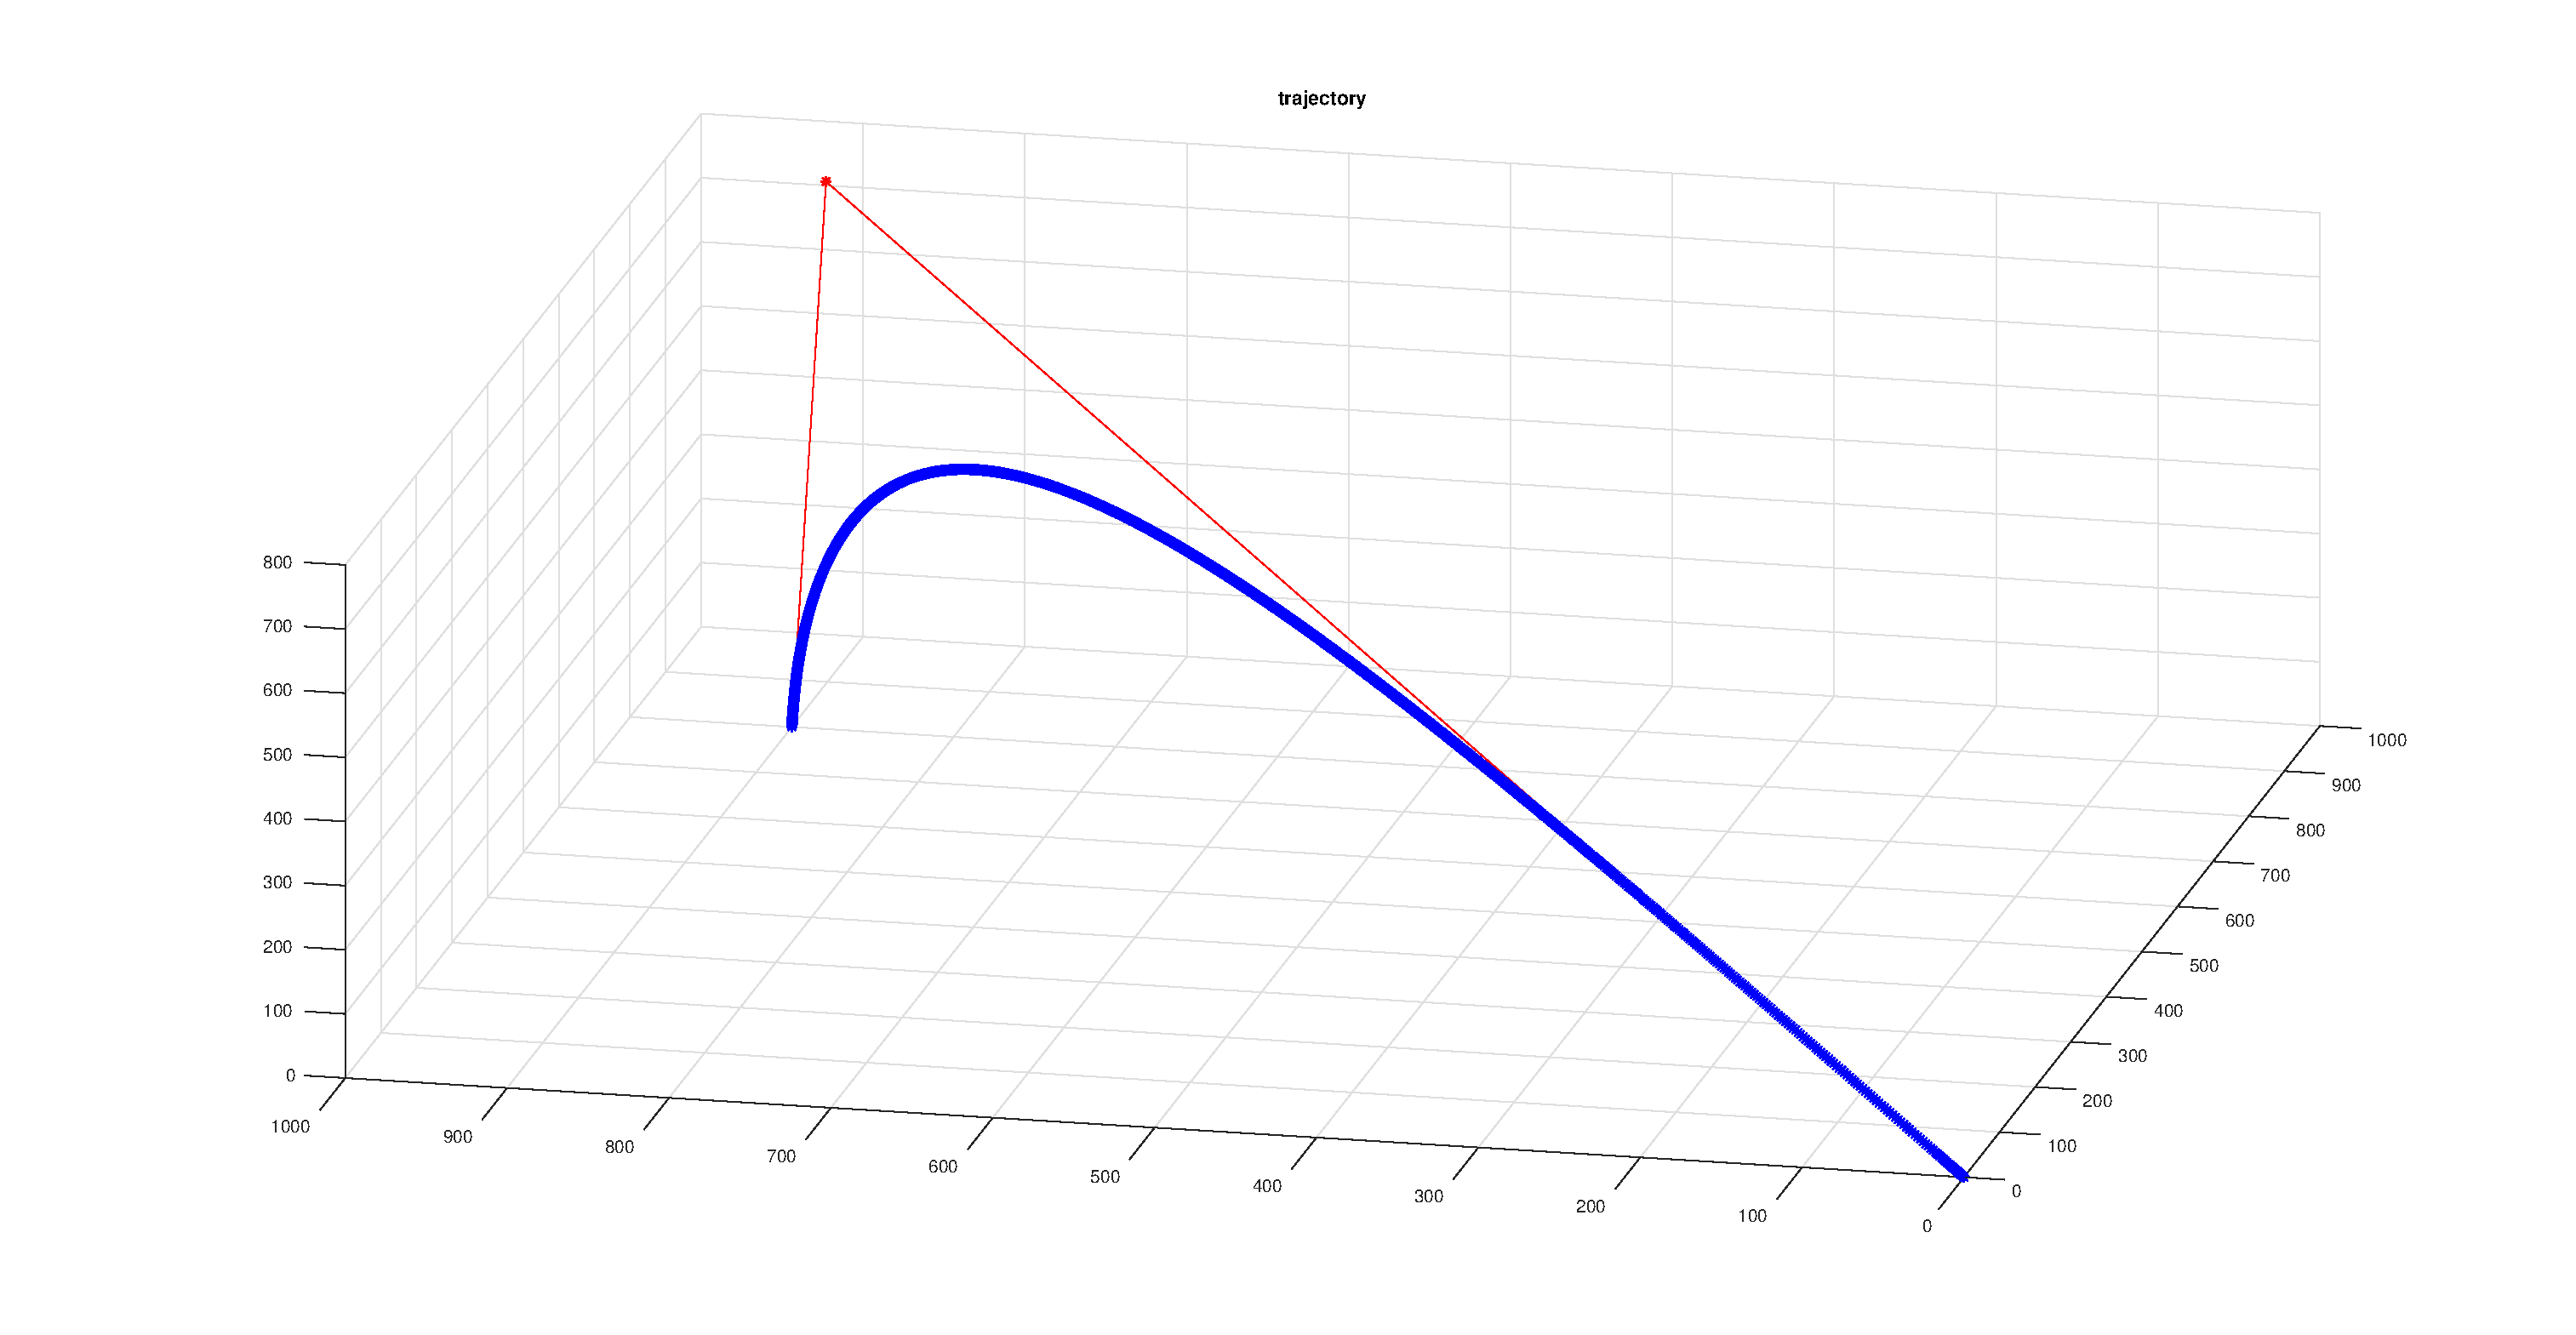
\includegraphics[height=0.6\textwidth]{motion_law_sample_problem_traj}
		\end{minipage}
		\caption[Motion Law Sample Problem]{Motion Law Sample Problem,
		left: problem layout, right: trajectory found}
		\label{fig:motion_law_sample_problem}
	\end{figure}

	\begin{figure}[hbt!]
		\centering
		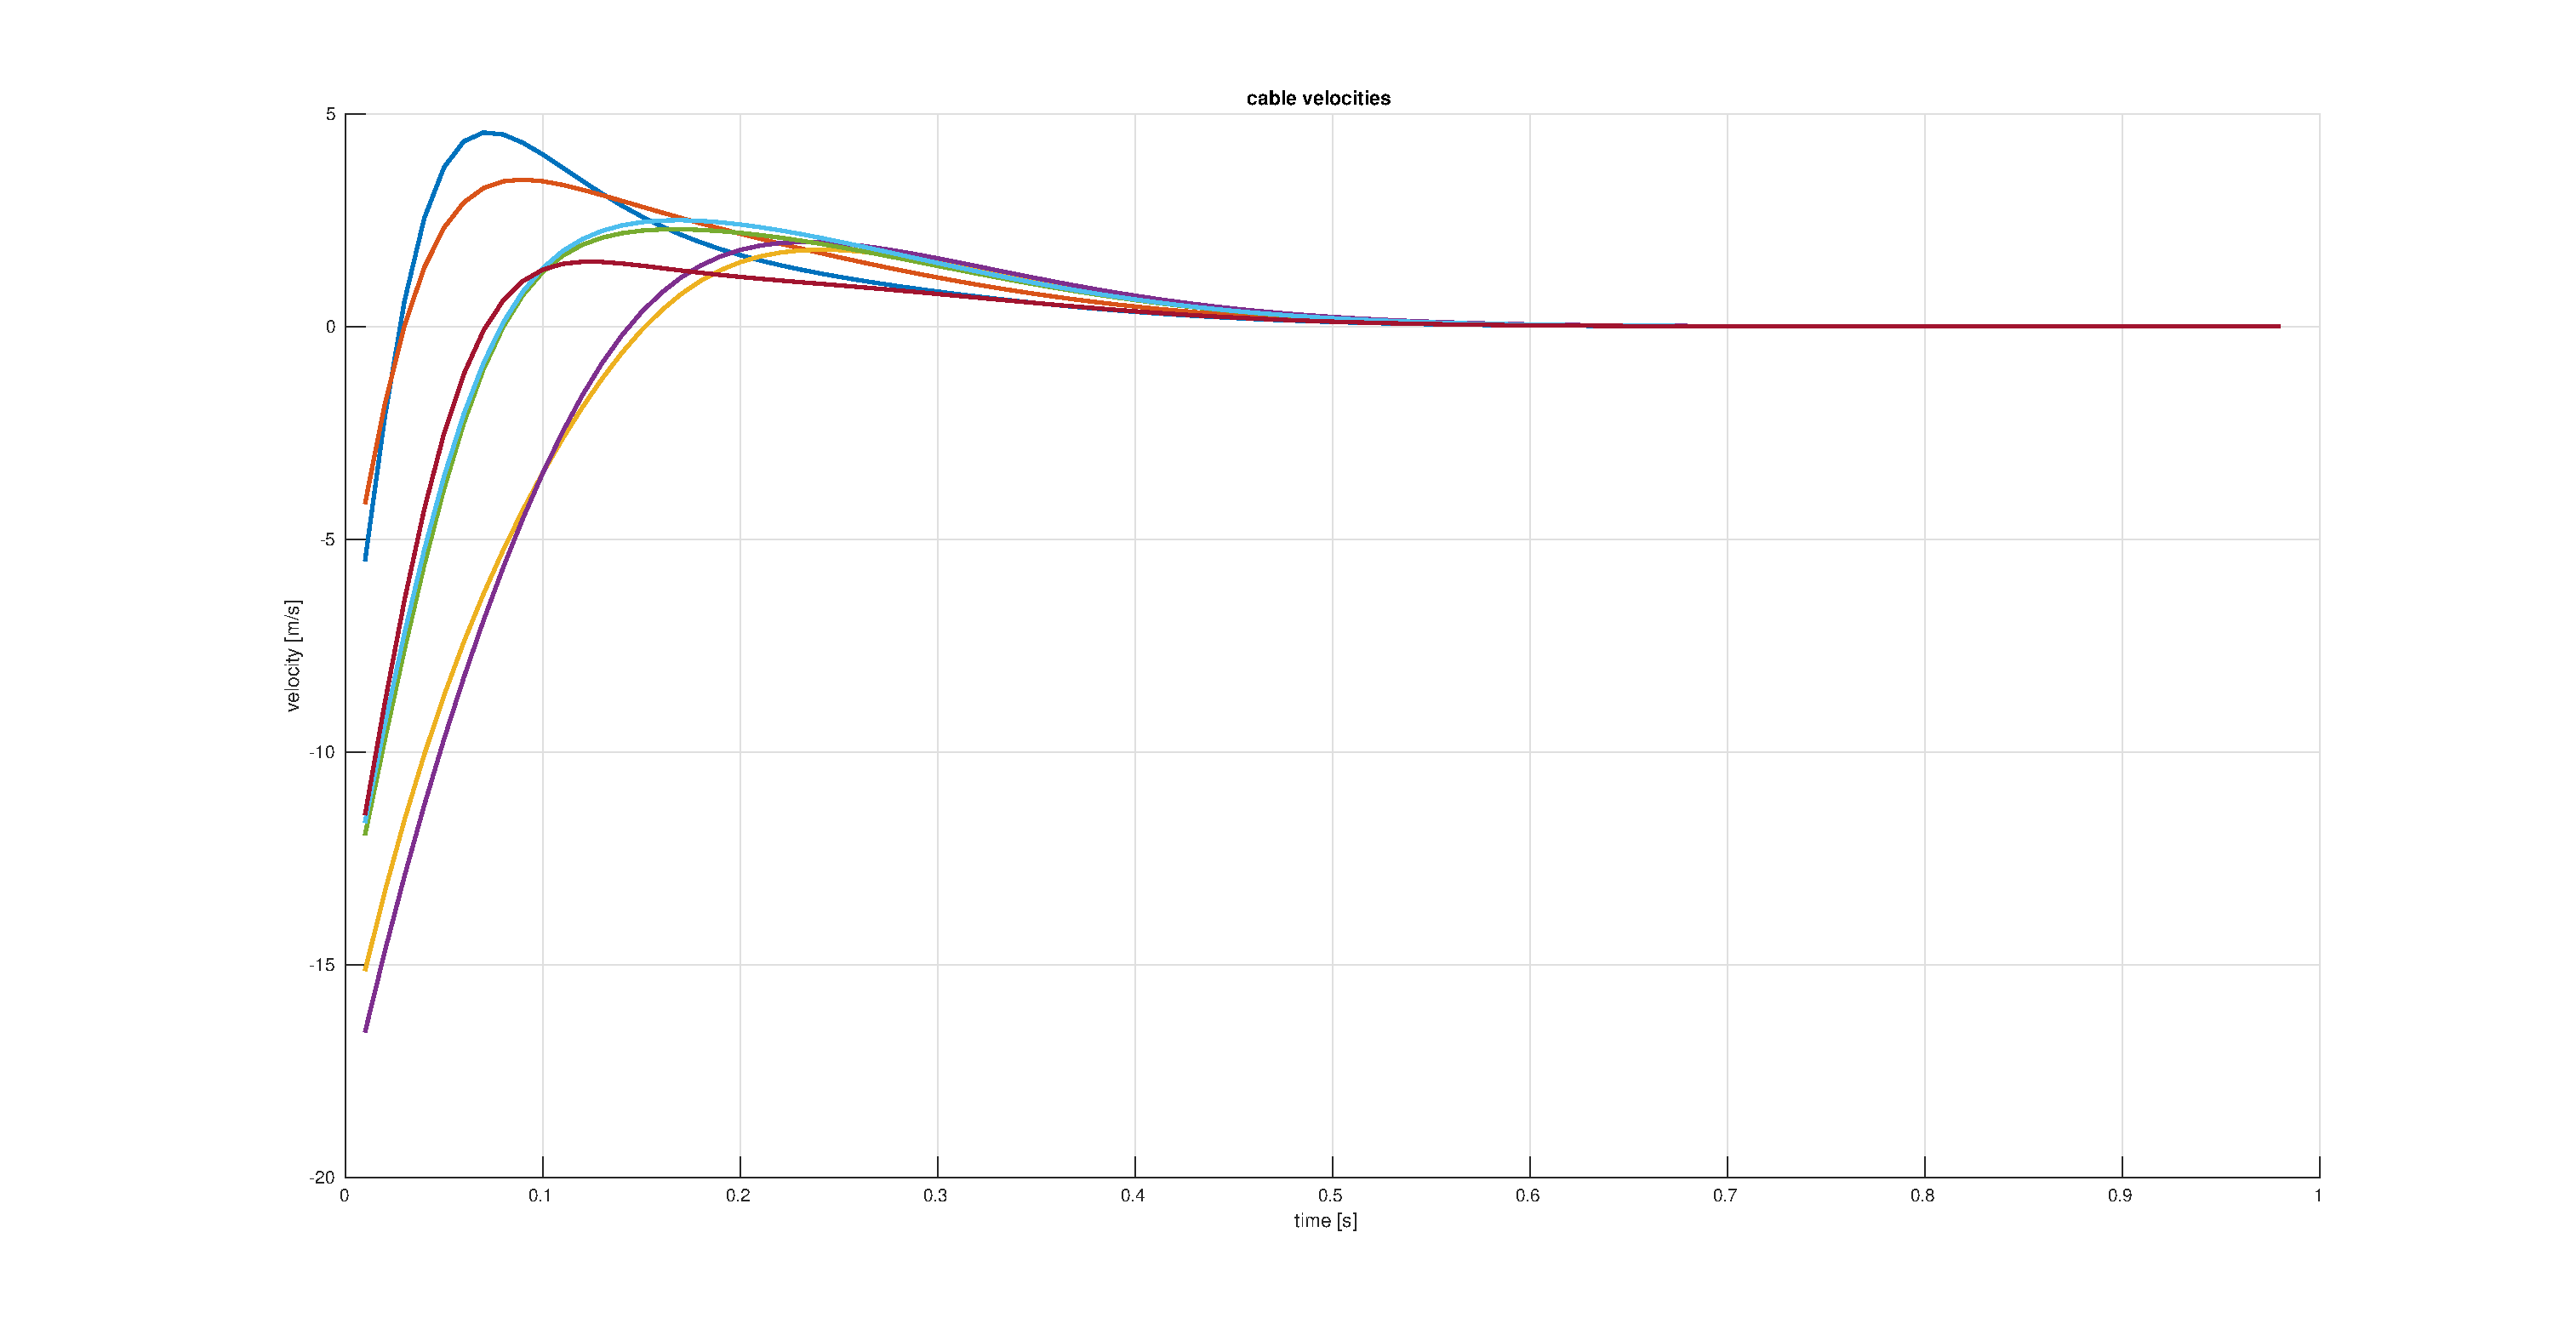
\includegraphics[width=\textwidth]{motion_law_base_velocities}
		\caption{Cable Velocities without Motion Law Scaling}
		\label{fig:cable_velocities_without_motion_law_scaling}
	\end{figure}

	\begin{figure}[hbt!]
		\centering
		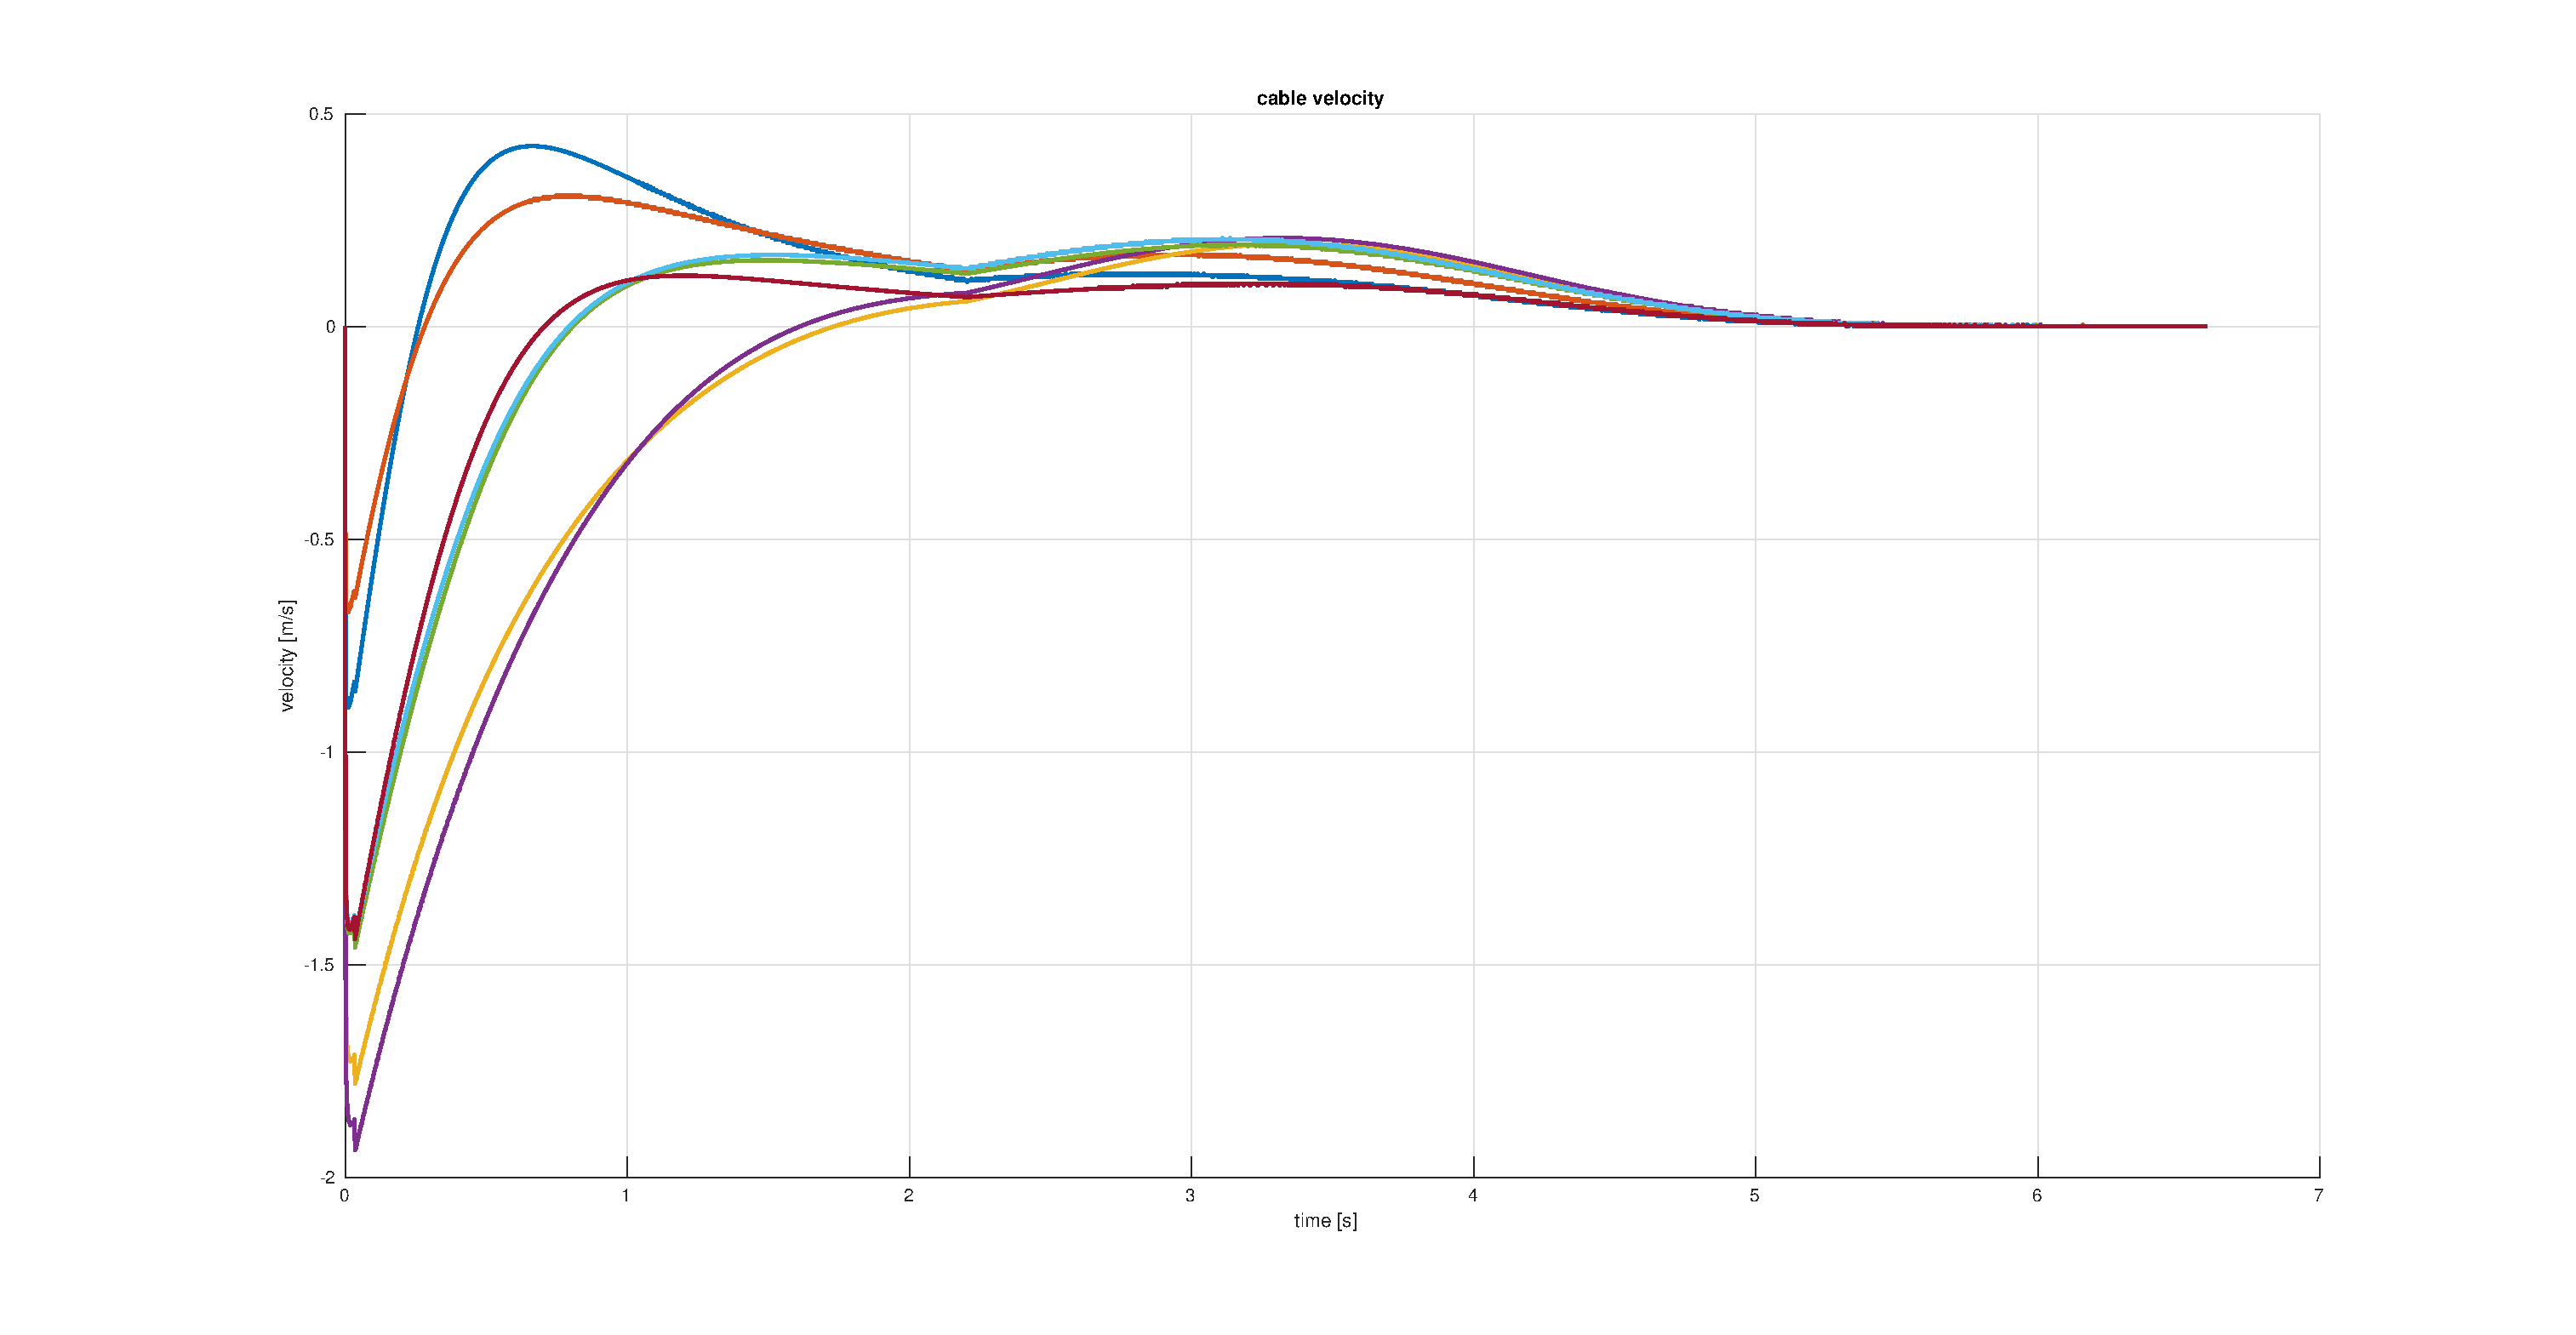
\includegraphics[width=\textwidth]{motion_law_output_velocities}
		\caption{Cable Velocities with Motion Law Scaling}
		\label{fig:cable_velocities_with_motion_law_scaling}
	\end{figure}

	\begin{figure}[hbt!]
		\centering
		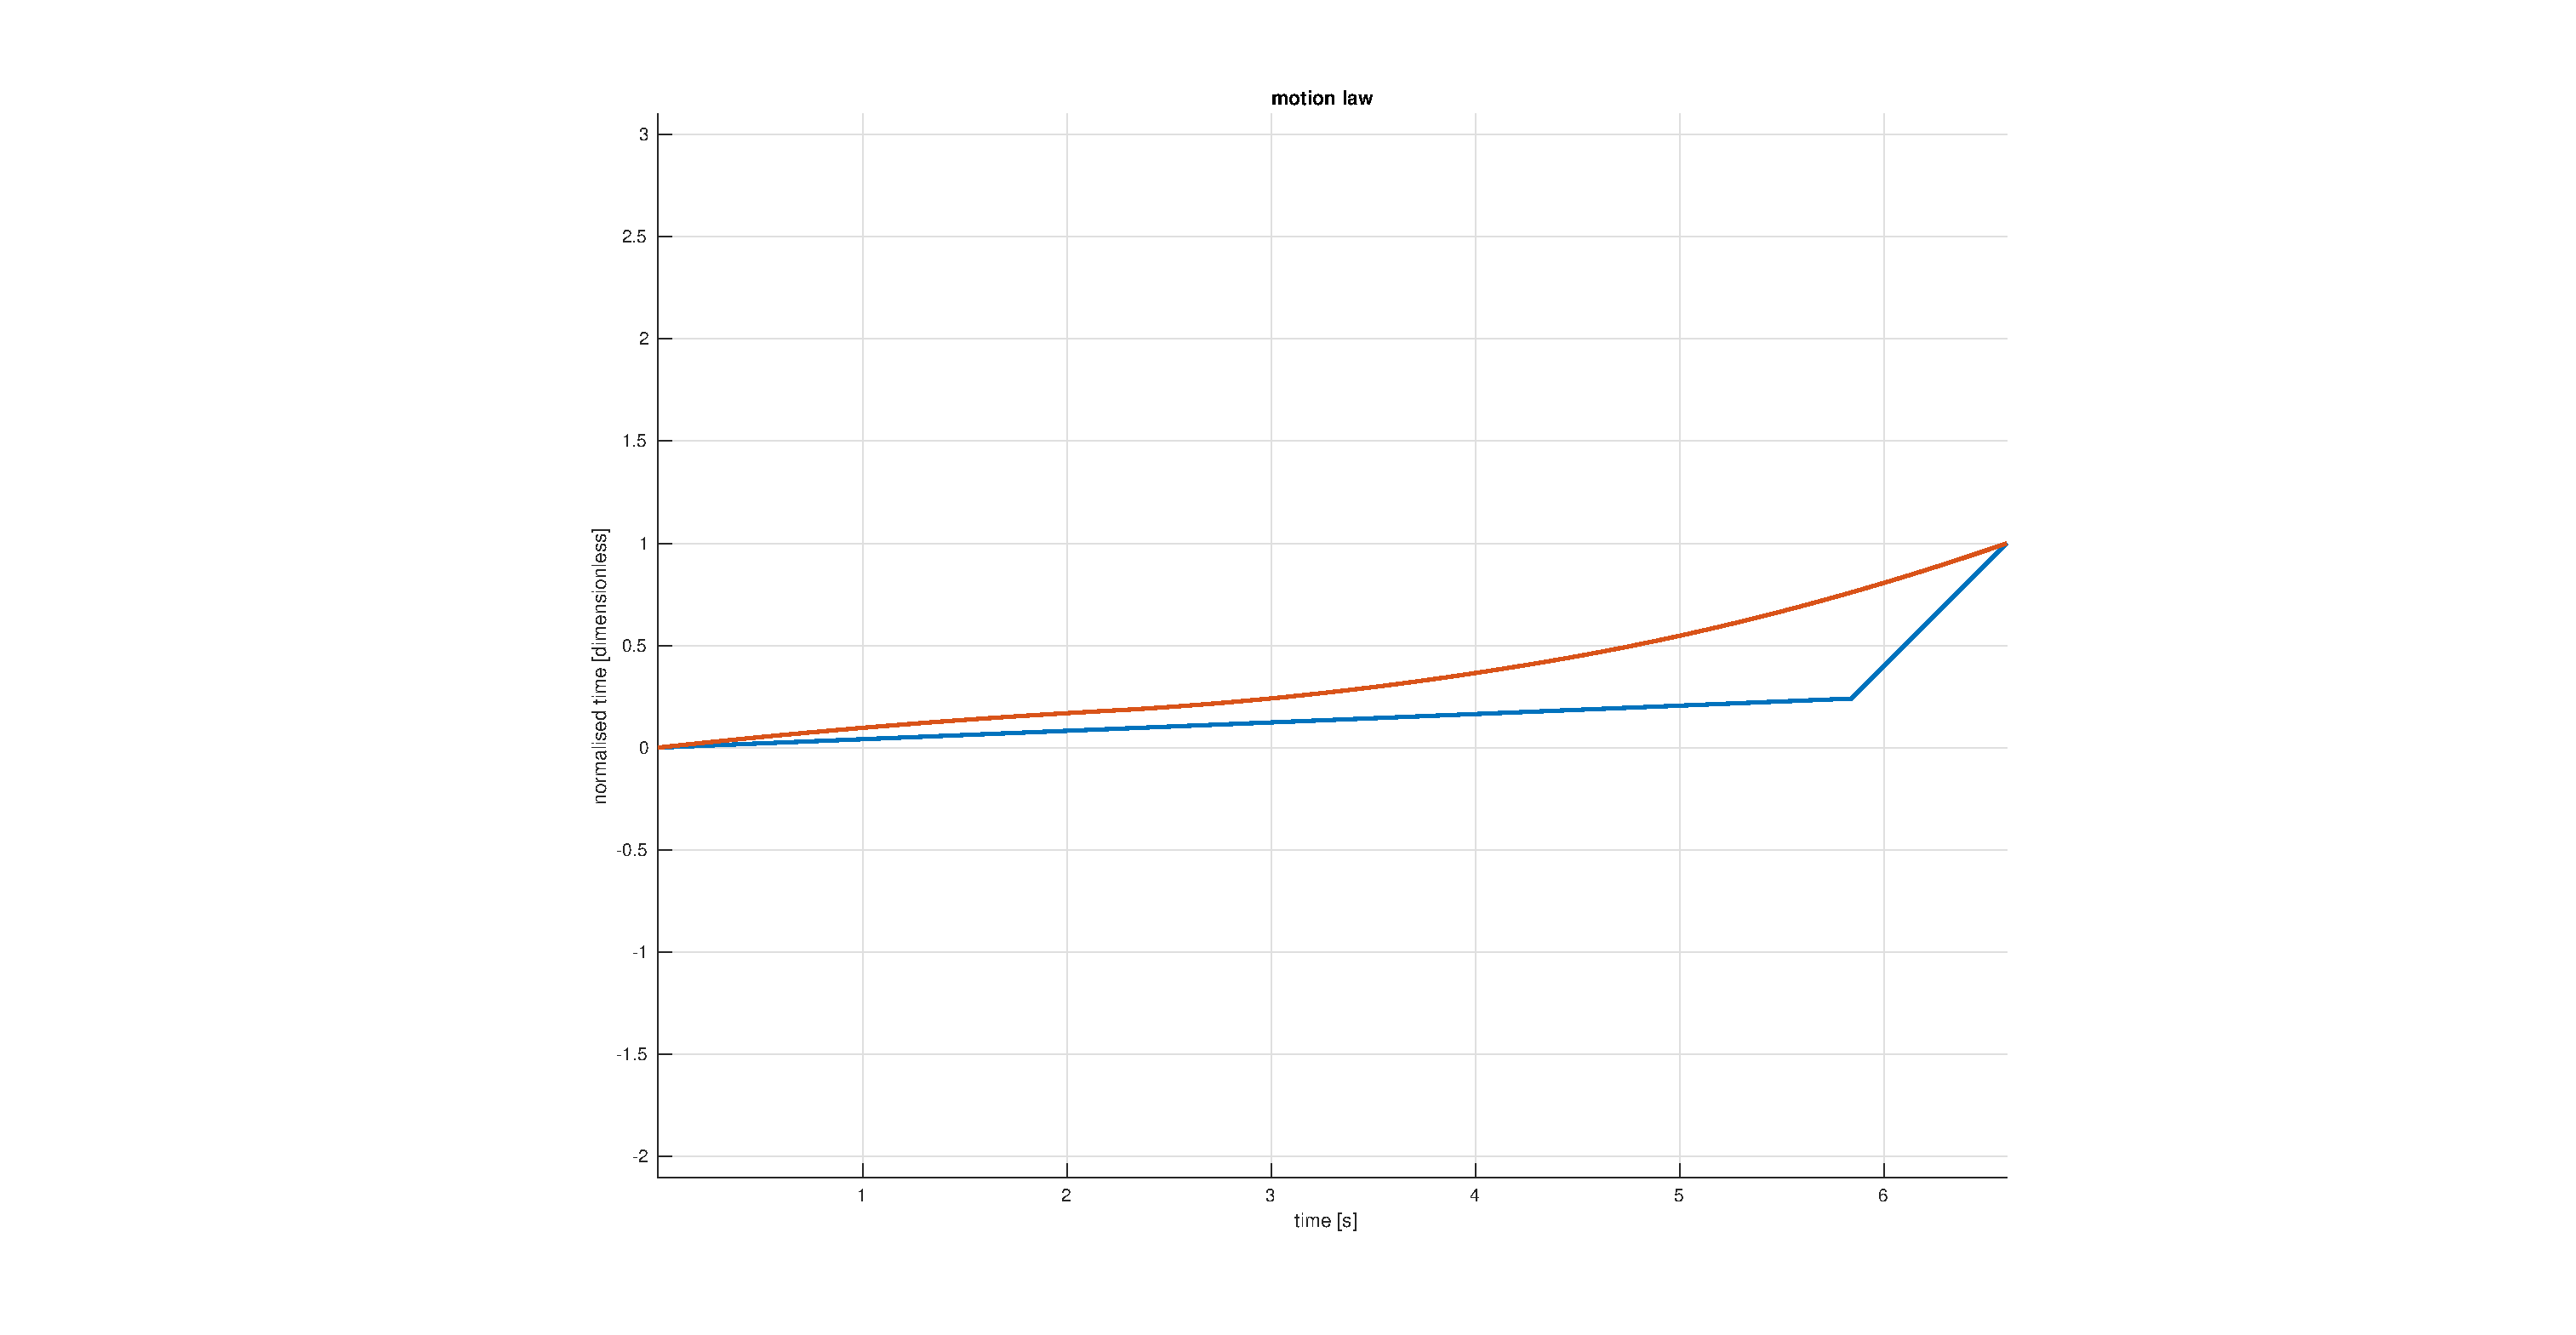
\includegraphics[width=\textwidth]{motion_law}
		\caption{Cable Velocities with Motion Law Scaling}
		\label{fig:motion_law}
	\end{figure}

	The output of the algorithm for this problem is shown in
	Figures~\ref{fig:cable_velocities_without_motion_law_scaling},
	\ref{fig:cable_velocities_with_motion_law_scaling} and~\ref{fig:motion_law}.
	In these figures, the algorithm attempted to find a motion law such that the
	maximum velocity does not exceed $2\si{\meter\per\second}$. For comparison,
	Figure~\ref{fig:cable_velocities_without_motion_law_scaling} shows the case
	where the algorithm is not applied ($\timesym \defeq \timenorm$). As can be
	seen, cable velocities reached up to $15\si{\meter\per\second}$ in this
	case. The motion law generated by the algorithm is reported in
	Figure~\ref{fig:motion_law}. In this figure both the control polygon and the
	B-Spline curve are shown. The output velocities found by applying this
	motion law is shown in
	Figure~\ref{fig:cable_velocities_with_motion_law_scaling}. As can be seen
	from the figurek the motion law succeeds in keeping the cables within their
	velocity bounds.


